\chapter{序論}
\label{chap:introduction}

\section{背景}
\label{section:background}

今日の音楽のリスニング環境は、イヤホンやヘッドホンで聴くことはごく当たり前のものになっている。スマートフォンやコンピュータといった再生機器に、3.5mmステレオミニプラグ\footnote{いわゆるイヤホンジャック}を接続するか、あるいはBluetoothといった無線伝送によってオーディオは伝送されている。

一般的な民生用オーディオ伝送では、インターフェイスや接続が手軽な利便性をとり、ある程度の音質劣化や遅延は許容されている。一方で、業務用オーディオの世界では妥協のない高音質の追求や、絶対に伝送される安定性が優先される。

プロのアーティストによるライブ、テレビ局やインターネットの動画配信などで用いられる業務用オーディオでは、民生向けで使われるオーディオ伝送に比べ、次にあげるような条件が要求される。

\begin{itemize}
  \item 高音質
  \item 低遅延
  \item 伝送の安定性
\end{itemize}

% ただし、オーディオ入力と出力の最初と最後は図\ref{fig:first_and_last_need_ad_da}のように、必ずアナログとデジタルの変換(以下、A/D変換、D/A変換)が必要となる。
デジタル伝送技術は、アナログ伝送に比べ伝送経路による劣化が起こりにくくなっている。ただし、オーディオ入力と出力の最初と最後は必ずアナログとデジタルの変換(以下、A/D変換、D/A変換)が必要となる。そのため、すべての伝送経路をアナログで伝送するのに比べ、少なからず伝送するにあたりA/D変換とD/A変換にともなう遅延が発生する。しかしながら、技術の向上によって遅延量は少なくなっている。
% たとえば、XXXでA/D、D/A変換に要する時間はX.Xms以内である。

% \begin{figure}[htbp]
%   \centering
%   \label{fig:first_and_last_need_ad_da}
%   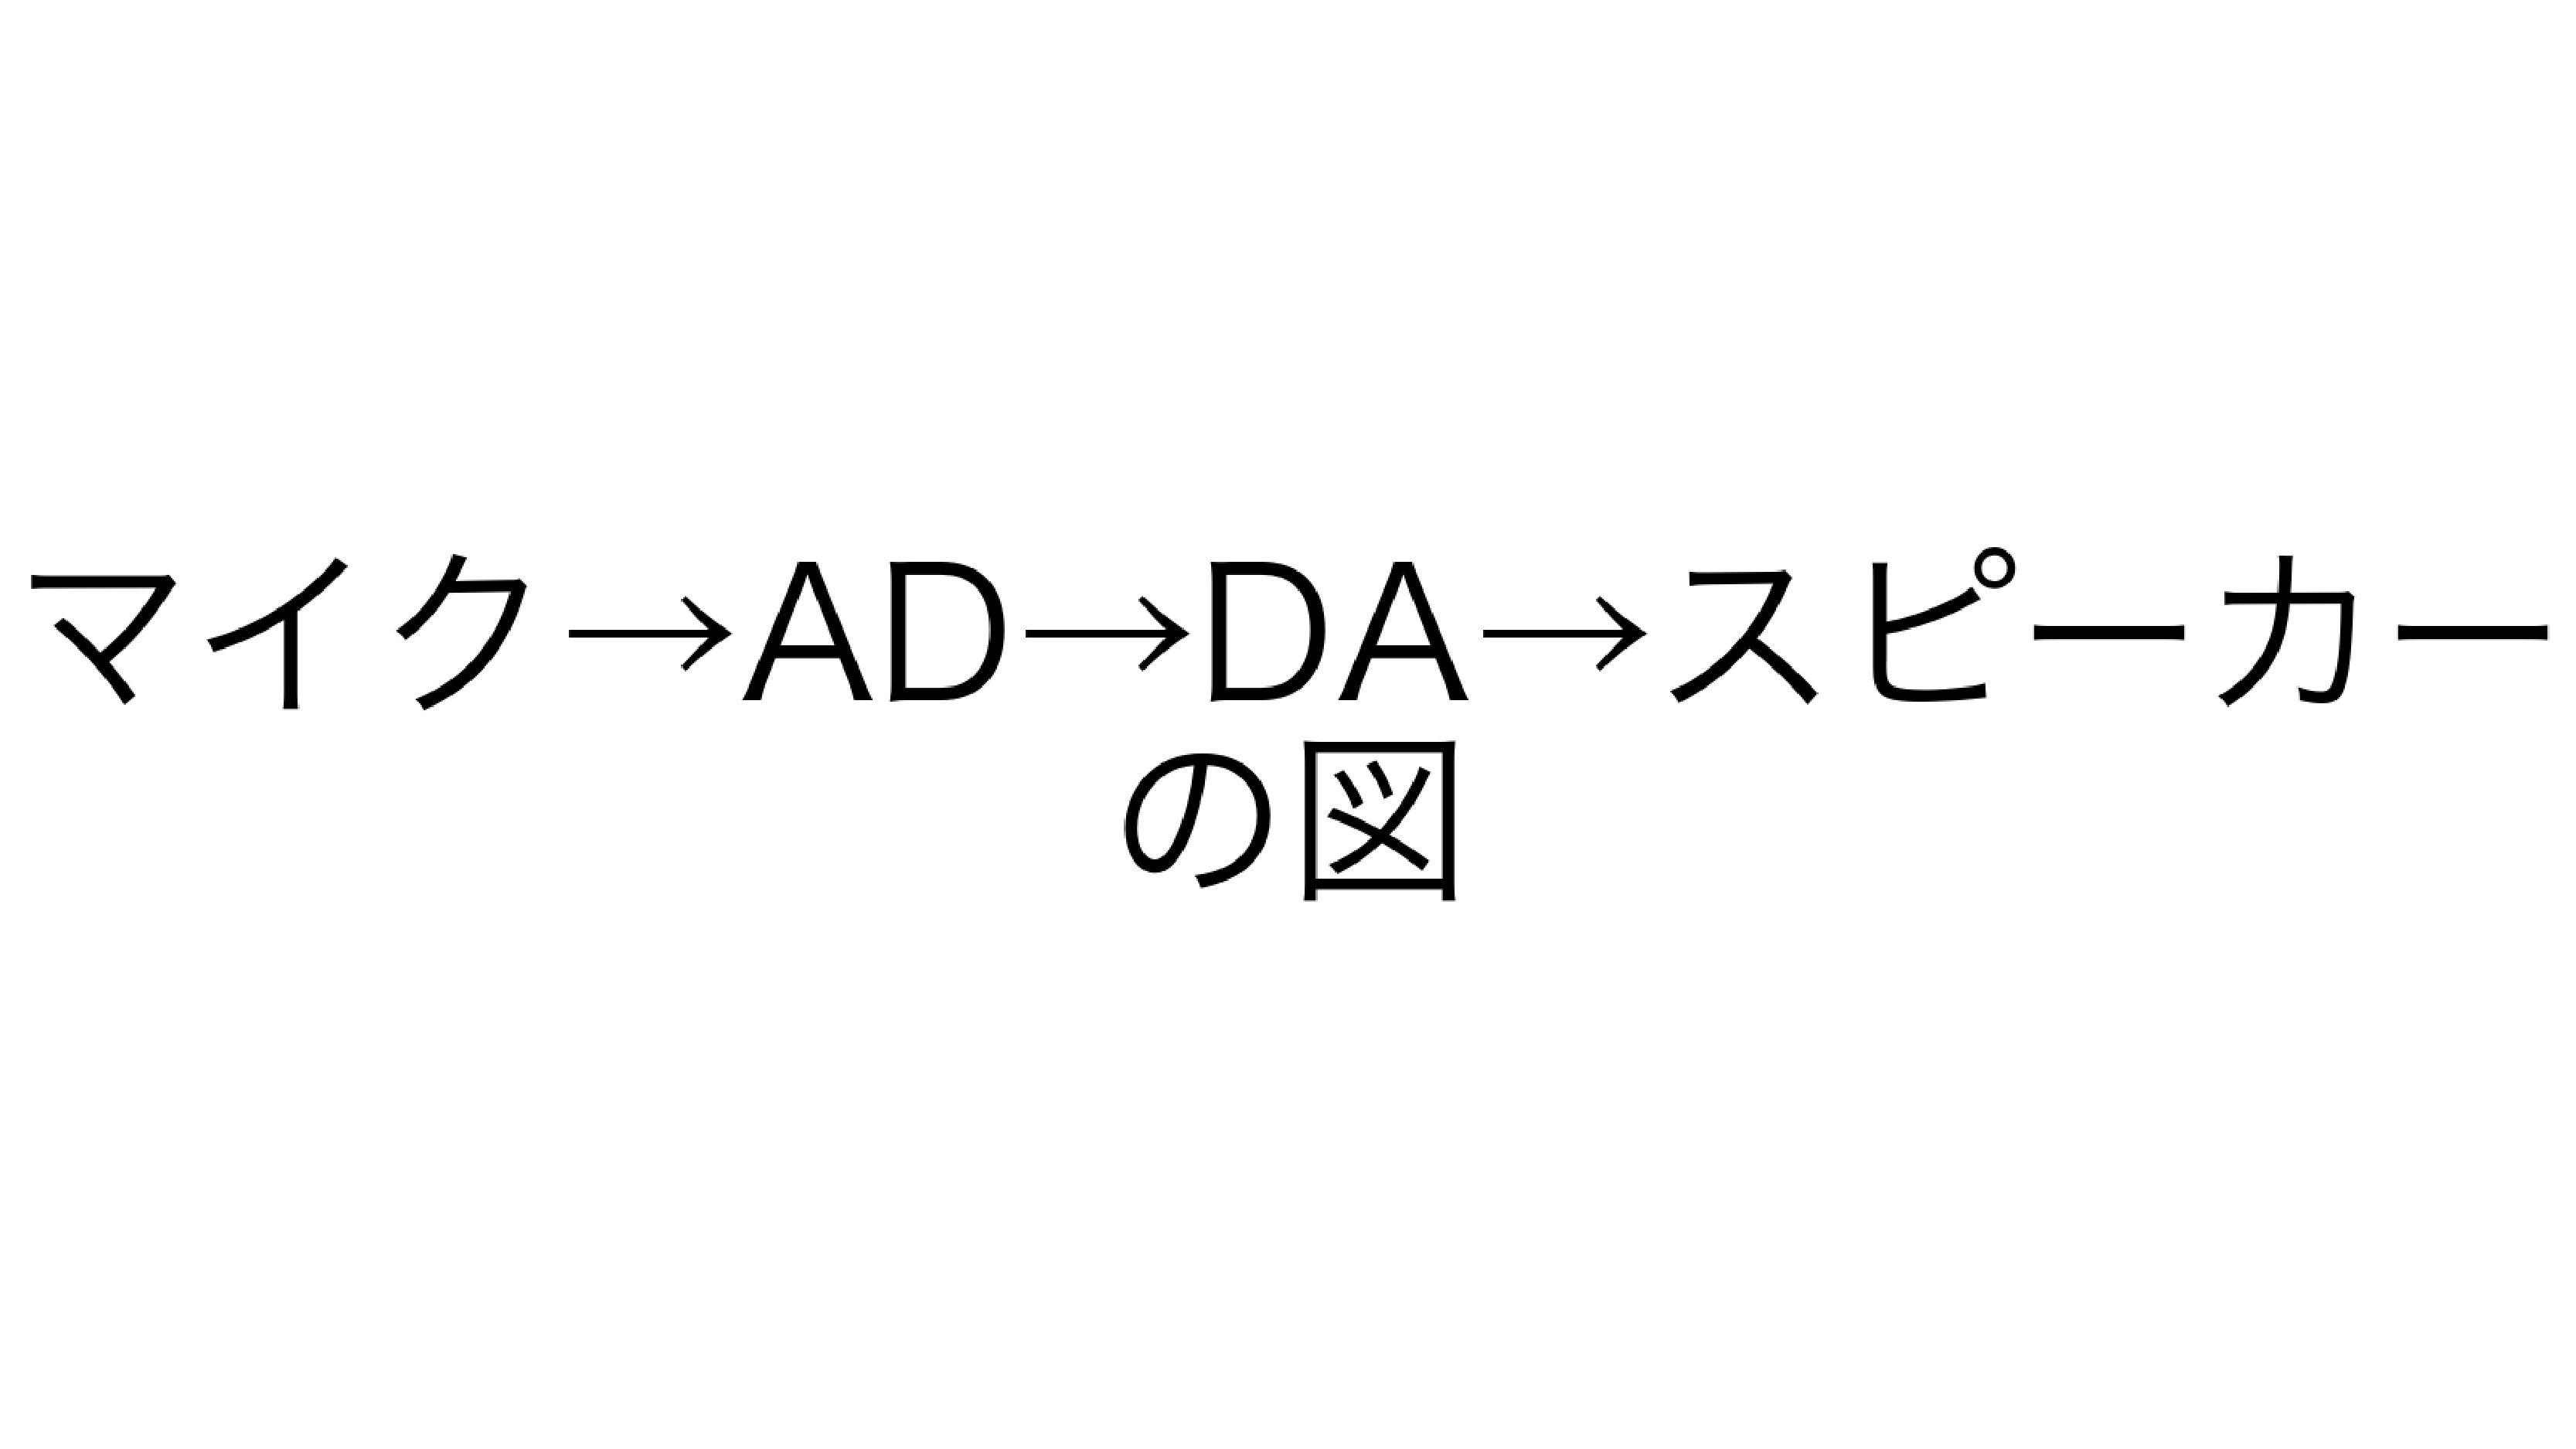
\includegraphics[width=0.8\linewidth]{img/first_and_last_need_ad_da.pdf}
%   \caption{マイク→AD→DA→スピーカーの図}
% \end{figure}

もう一つ、デジタル伝送を行うことによる恩恵は高音質のまま伝送できることである。アナログ伝送のまま伝送を行えば、理論的にはA/D、D/A変換を挟まないため、劣化しないはずである。しかしながら、アナログ伝送は外部からのノイズに弱く、伝送経路中で劣化する可能性が否定できない。

そこで、デジタル伝送ではアナログ信号を0と1の信号にする。アナログ信号は、連続したデータ表現のため、デジタル信号にそのまま表現すると無限となってしまう。それでは現実的でないためデジタル信号では、量子化によってデータ量を減らすことができる\cite{analog-io}。したがって、従来アナログ伝送においてケーブル1本で1チャンネル伝送していたところをデジタル伝送により2チャンネル以上の多チャンネル伝送ができるようになる。AES/EBUというデジタル伝送規格では、接続に用いるケーブルにもよるが2〜16チャンネル程度の伝送が行える。
% 要出典

インターネット、ネットワークの接続に利用するEthernet(イーサネット)は、インターネットの高速化やコンピュータで扱うコンテンツのリッチ化にともない、通信速度の高速化が進んでいる。2019年現在、市販のEthernetケーブルを用いた接続では、最大10Gbps\footnote{Gbps: Gigabit per second、ギガビット毎秒}の通信速度で転送することができる。

% (余裕があればAES/EBUの転送速度と比較する)

% \begin{figure}[htbp]
%   \centering
%   \label{fig:ethernet_cable}
%   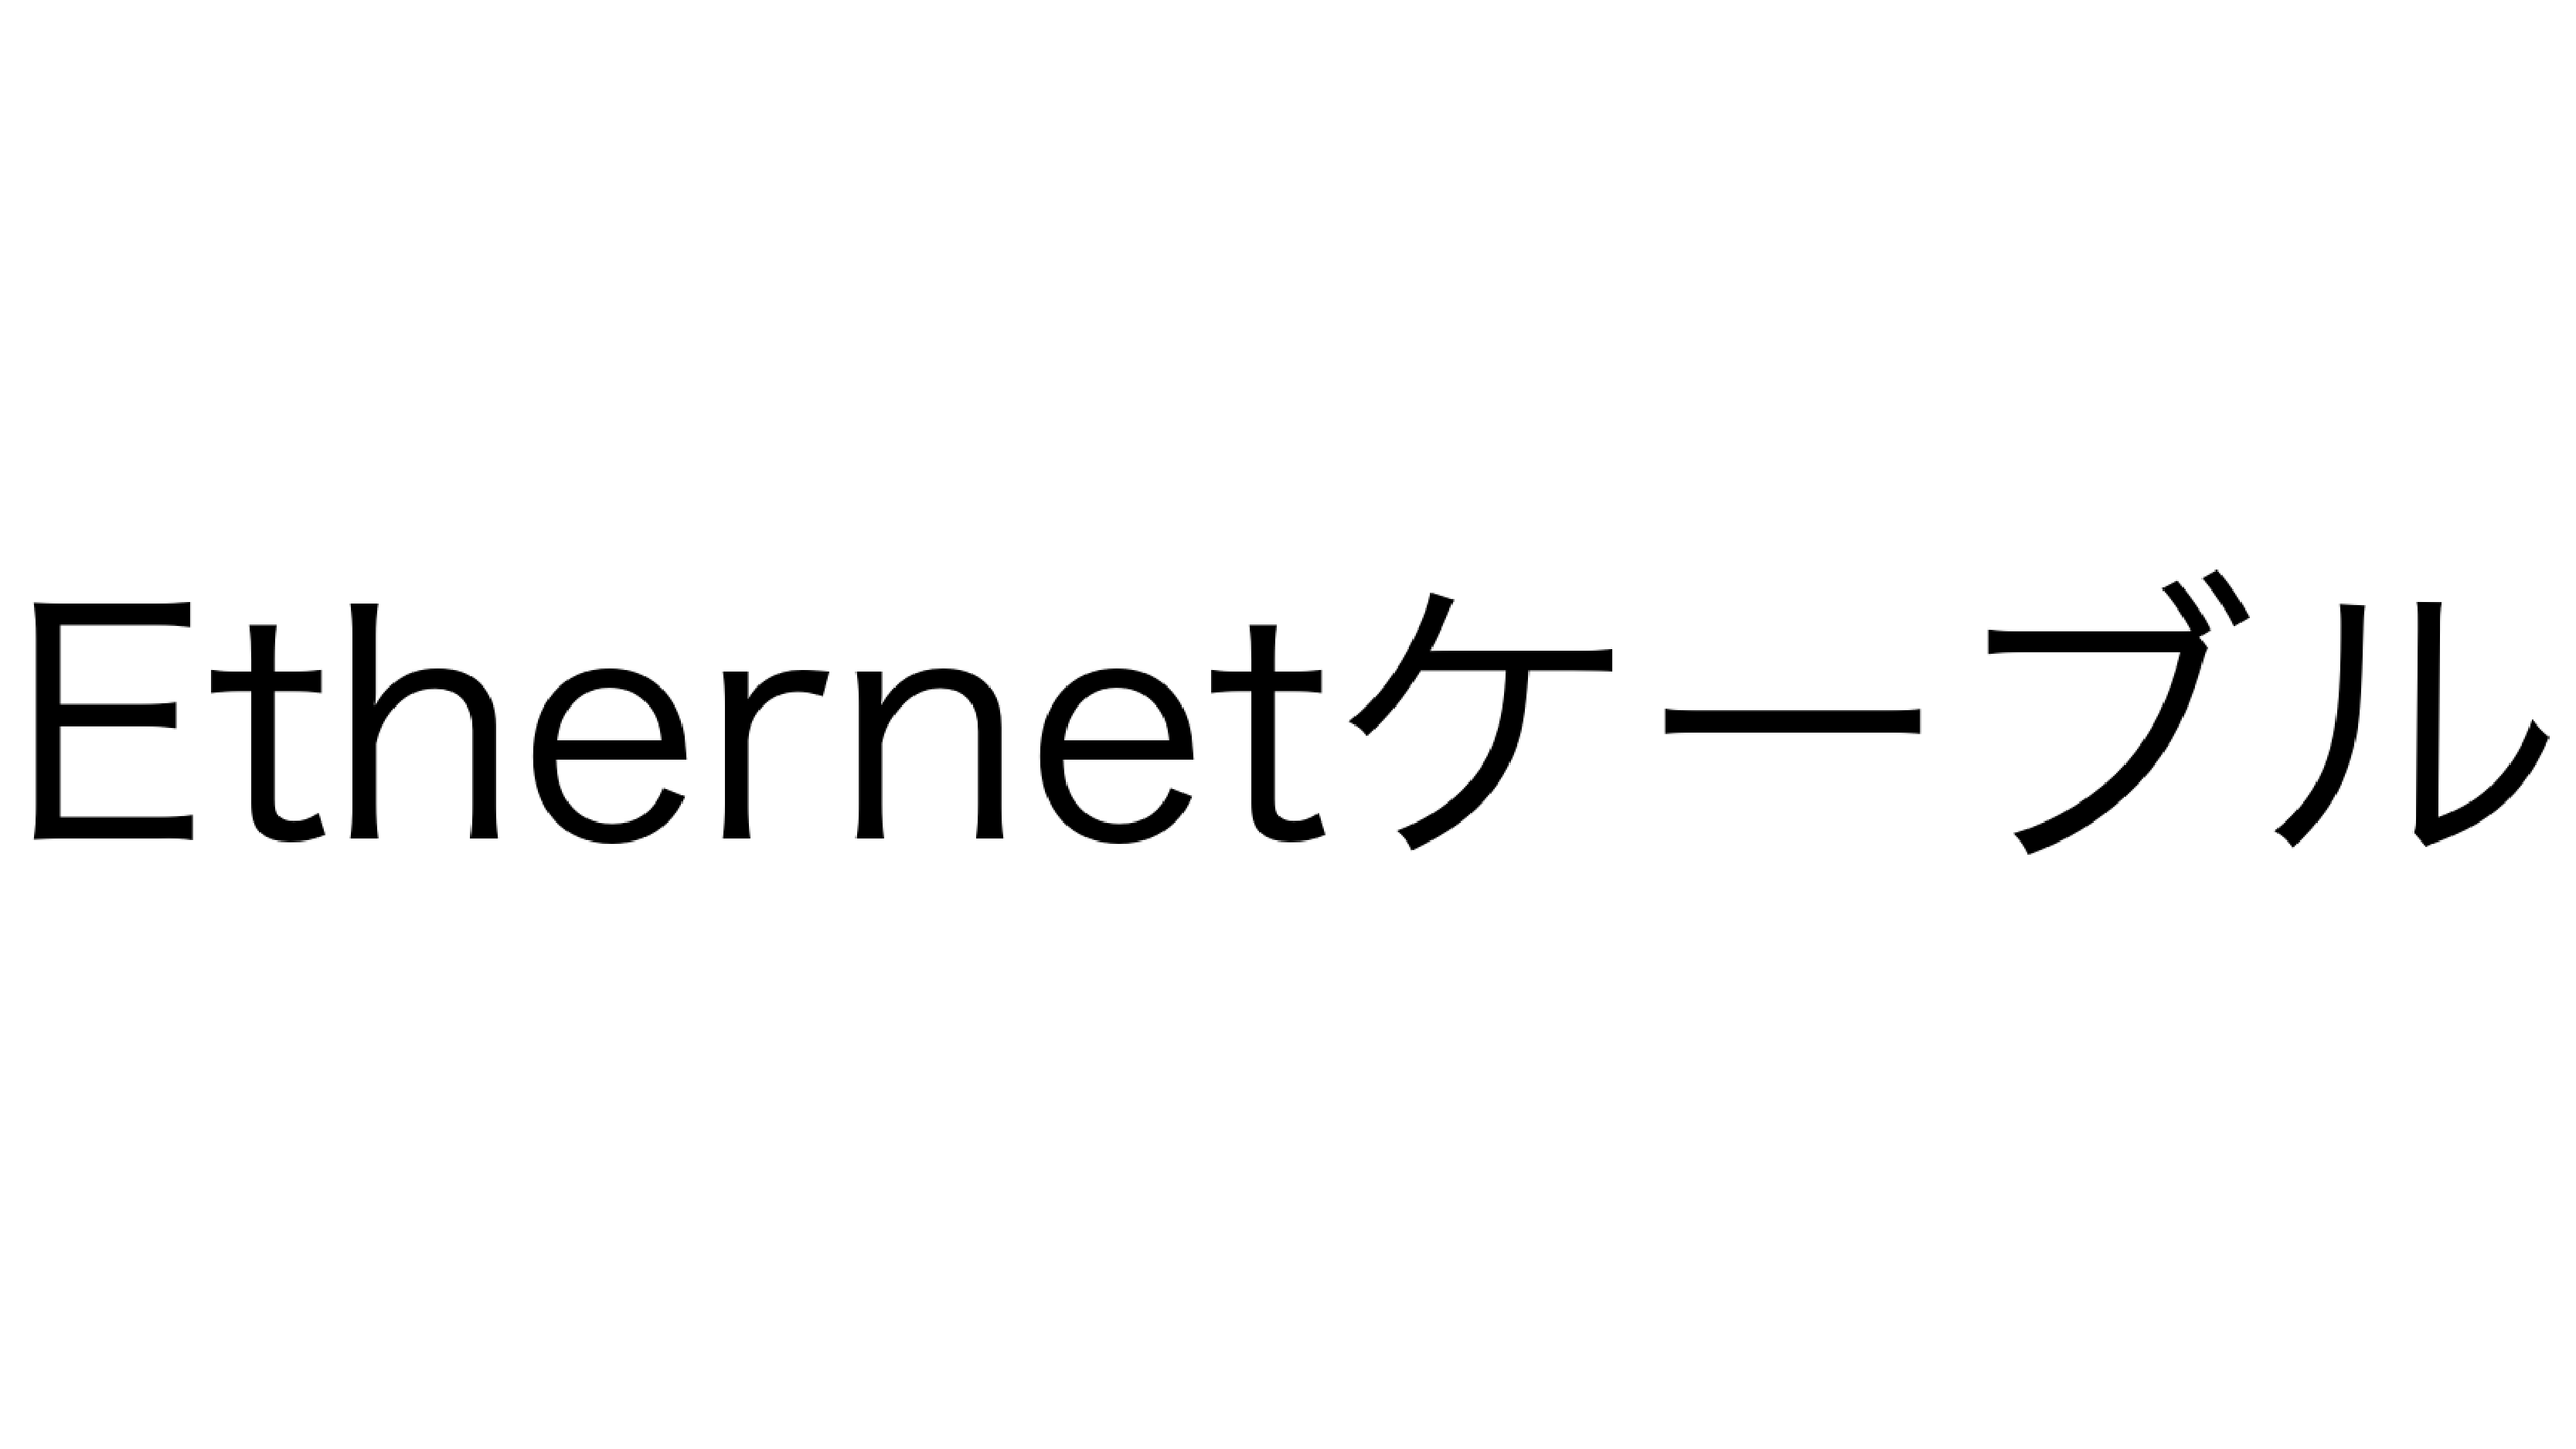
\includegraphics[width=0.4\linewidth]{img/ethernet_cable.pdf}
%   \caption{Ethernetケーブル}
% \end{figure}

Ethernetを用いたデジタルオーディオ伝送では、高速なEthernetの帯域を用いて従来のデジタルオーディオ伝送に比べ、より多くのチャンネルを伝送することができる。多チャンネル化が実現できるのみならず、IPベースのエラー訂正が可能となる。

大規模な業務用オーディオ環境では、広帯域なEthernetを用いたIPベースの伝送への移行が進んでいる。主流となっているのは、Audinate社が開発したDanteという規格だ。Audinate社はDante機能のチップをオーディオ機器メーカーに卸す手法をとっている。オーディオ機器メーカーに対してDanteに関する詳細な仕様は公開されておらず、ブラックボックスとなっている現状がある。したがって、オープンなIPベースのデジタルオーディオ伝送が必要である。

そこで、登場したのがAES67だ。AES67は、乱立する既存のIPベースのデジタルオーディオ伝送技術を共通化し、相互運用性を高めるための規格である。今後、オーディオのIP伝送が主流となっていくなかで、オープンな標準化技術によってさまざまなオーディオ機器を接続できることは重要である。

\section{本論文の目的}

本論文では、オーディオ機器の最初と最後のA/D、D/A変換を行う前のアナログ伝送を除くすべての伝送経路をAES67によって実現できるかの可能性を追求する。必要となる、AES67オーディオストリームを送受信するアプリケーションを実装する。その上で、既存の商用規格から置き換えが可能なのか、業務用途で要求される厳しい条件に耐えられるかを検証する。

\section{本論文の構成}

本論文における以降の構成は次の通りである。

\ref{chap:related_works}章では、本論文で扱うIPベースのオーディオ伝送について理解ための前提技術について、解説する。業務用オーディオが使われている現場の構成、さらにはオーディオのデジタル伝送技術について触れる。

\ref{chap:design}章では、AES67を用いたIPベースのオーディオ伝送の送受信を行うアプリケーションの設計を行い、その内容について述べる。

\ref{chap:implementation}章では、\ref{chap:design}章で設計したアプリケーションを実装し、その内容について述べる。

\ref{chap:evaluation}章では、\ref{chap:implementation}章で実装したアプリケーションをもとに、実際の業務用オーディオ環境を模した実験を行い、評価した結果について述べる。

\ref{chap:conclusion}章では、本研究における結論と今後の展望、業務用オーディオの伝送技術の未来について述べる。
